\subsection{Observed TCEs}

\label{tces}
As with the previous three Kepler planet candiate catalogs \citep{Coughlin2016,Mullally2015cat,Rowe2015cat}, the population of events that were used to create KOIs and planet candidates are known as Threshold Crossing Events or \opstce s.  These are periodic dimmings of a light curve that were found by the Transit Planet Search module and validated by the Data Validation module of the Kepler pipeline INSERT Jenkins2017kdph REF \citep{Fanelli2011}.   The Data Release 25 \opstce s were created by running the SOC 9.3 version of the pipeline on the Kepler DR25, Q1--Q17 \Kepler\ PDC time-series.  For a thorough analysis of the DR25 TCEs and on the pipeline's search see \citet{Twicken2016}.  

The DR25 \opstce s, their ephemerides, and the metrics calculated by the pipeline are available at the NASA Exoplanet Archive \citep{Akeson2013}.  In this paper we endeavor to disposition these signals into planet candidates and false positives.   Because the \opstce s act as the input to our catalog, we first describe some of their properties as a whole and reflect on how they are different than the previous \Kepler\ TCE table.

We have plotted the distribution of the \ntcesnorogue\ \opstce s in terms of period in Figure~\label{f:tces}. Notice, an excessive number of short and long period \opstce s with the number increasing with decreasing MES. 

As with previous catalogs, the short period ($<10$\,d) excess is dominated by true, sinusoidal variability of the star. The long period excess is dominated by instrumental noise. For example, a decrease in flux following a cosmic ray hit (a.k.a. SPSD, Sudden Pixel Sensitivity Drop-out), can match-up with natural fluctuations in the data to produce a TCE. Also, image artifacts known as rolling-band is very strong on some channels INSERT KDCH REF\citep[see page][]{KDCH}  and since the spacecraft rolls every 90\,days, causing a star to roll onto a \Kepler\ channel with significant rolling band, these variations can easily line-up to produce TCEs at 370\,d. This is the spike in the \opstce\ population seen in Figure~\ref{f:tces}. This excess of long period TCEs is significantly larger than in the DR24 catalog \citep{Seader2015}. Most likely, this is because DR24 implemented an aggressive and irregular veto known as the bootstrap metric \citep{}INSERT JENKINS KSCI HERE.  For DR25 this metric was calculated INSERT JENKINS2016 REF, but was not used as a veto.  Also other vetos were tuned down causing more TCEs across all periods to be created.  %\citep{Jenkins2016},

To summarize, for DR25 the number of false signals among the \opstce s  is drastically larger than in any previous catalog. As a result, we expect the \opstce\ list to contain more true exoplanets than before. However, the reliability of the \opstce\ catalog is lower than it has been in the past.   

\begin{figure*}[h!]
 \begin{center}
  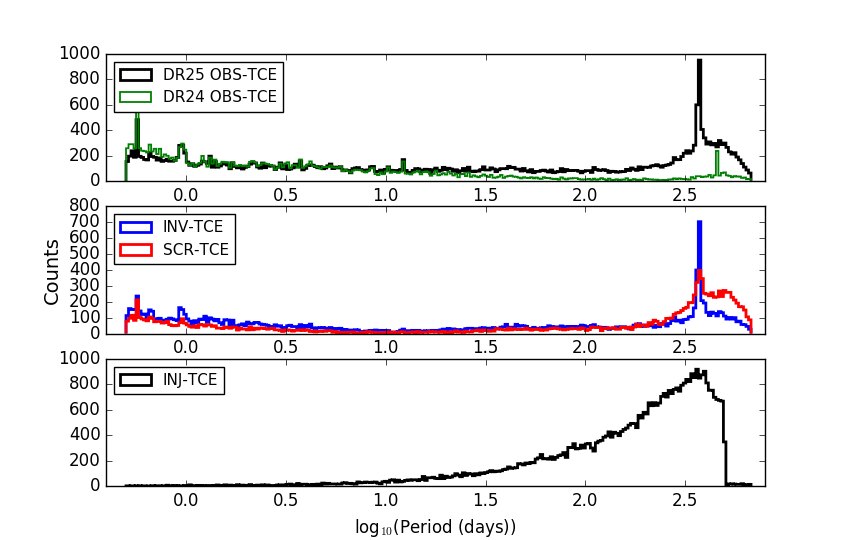
\includegraphics[width=1.1\linewidth]{fig-tcePeriods.png}
  \caption{\ref{f:tces} Histogram of the log$_{10}$(period) in days of the four different TCE populations used to create this catalog. In the top plot the DR24 OBS-TCE population is shown for reference.}
  %\caption{\ref{f:tces} A two dimensional histogram of the number of TCEs by log(period) and log(MES). The marginalized distributions for log(period) and log(MES) are projected along their respective axes and shown on the top and right respectively. }
 \end{center}
 \end{figure*}



\subsection{Rogue TCEs}
The DR25 TCE table at NExScI contains \ntces\ DR25 Observed TCEs (\opstce s), however, in this paper we disposition \ntcesnorogue\ of these \opstce s. The remaining \opstce s are known as ``rogue" TCEs, and were created because of a bug in the Kepler pipeline which let through certain three-transit events. Because the primary purpose of this catalog is to be able to accurately calculate occurrence rates and because this same bug was not present when characterizing the completeness of the \Kepler\ Pipeline \citep{}BURKE PRODUCT REFERENCE, we ignore the rogue TCEs here. For more information see the documentation for the occurrence rate products INSERT BURKE2017 REF% \citet{Burke2017} .
Also note that all of the TCE populations (INJ, INV, SCR and OPS, see the next section) had this problem. For this catalog paper we are only considering the non-rogue TCEs.